\documentclass[letterpaper,twocolumn,10pt]{article}
\usepackage{times}
\usepackage{helvet}
\usepackage{courier}
\usepackage{graphicx}
\usepackage{booktabs}
\usepackage{hyperref}
\usepackage{amsmath,amssymb}
\usepackage[font=small,labelfont=bf]{caption}
\usepackage[letterpaper,margin=0.75in]{geometry}
\frenchspacing
\setlength{\pdfpagewidth}{8.5in}
\setlength{\pdfpageheight}{11in}
\setcounter{secnumdepth}{0}
\setlength{\textfloatsep}{7pt plus 1pt minus 2pt}
\setlength{\floatsep}{6pt plus 1pt minus 2pt}
\setlength{\intextsep}{6pt plus 1pt minus 2pt}
\setlength{\abovecaptionskip}{3pt}
\setlength{\belowcaptionskip}{0pt}
\title{MaskShift: Forecasting Under Missingness-Mechanism Shift}
\author{Anonymous Submission}
\date{}

\begin{document}
\maketitle

\begin{abstract}
Forecasting papers commonly stress-test missing inputs by varying how many observations are removed. Deployment failures often vary a different quantity: why observations disappear. A weather station can stop reporting during storms, traffic detectors can go dark during congestion, telemetry can vanish under overload, and retired sensors can disappear permanently. These mechanisms can have the same missing rate while inducing different conditional mask laws. We study this failure mode as \emph{missingness-mechanism shift}. MaskShift is not a new forecasting backbone. It is a benchmark and theory paper showing that matched missing rate is not a sufficient robustness certificate for deployment missingness. We define a controlled encoder-mask protocol, generate matched-rate MCAR, block, value-triggered, volatility-triggered, blackout, and retirement masks, and evaluate forecast risk and model-ranking stability. On Weather and Electricity, mechanism identity explains large degradation variance and can reverse model rankings; Traffic and AirConvection are mixed and are reported as limits. With official TSLib PatchTST and TimeXer model classes under a custom MaskShift encoder-mask loop, maximum degradation over operational mechanisms is 135.8\% on Weather and 128.6\% on Electricity over three seed offsets, with worst Kendall $\tau=-1.0$ in both datasets. We additionally adapt official ChannelTokenFormer\_missing and S4M. ChannelTokenFormer\_missing gives mixed missing-aware evidence, while S4M is a useful negative/contrastive baseline under the reduced MaskShift protocol. A typed-head correction does not pass our claim gate, so we report it as a negative diagnostic. The central contribution is a reproducible audit protocol and evidence that missingness topology and conditional mask mechanism should be first-class benchmark factors.
\end{abstract}

\section{Introduction}

Time-series forecasting systems are usually evaluated on clean histories or on histories corrupted by simple missingness processes. This is convenient but brittle. In deployed systems, missing values are rarely neutral. A sensor missing at random, a sensor missing during high values, a cluster missing during a blackout, and a channel missing after retirement all give the forecaster a different piece of information. The observed value tensor can be matched in size and the overall missing rate can be matched, yet the mask itself has changed meaning.

This paper studies a narrow question: does robustness under MCAR or uniform block missingness certify robustness under deployment missingness? We argue and empirically show that the answer is no. The problem is not only that fewer values are observed. The problem is that the conditional law of the mask has shifted. In notation, the deployment distribution changes from a training or selection mechanism $p_A(M\mid X)$ to a deployment mechanism $p_B(M\mid X)$, while the marginal missing rate may remain fixed. A forecaster selected under $A$ can therefore be evaluated under a different conditional predictor at test time.

MaskShift is deliberately scoped as a benchmark/theory paper. It does not propose a new forecasting architecture, does not claim state-of-the-art clean forecasting accuracy, and does not claim that a lightweight typed correction solves missing-data forecasting. Instead, it contributes a failure-mode audit: controlled mask generators, rank-reversal metrics, degradation statistics, and a claim-to-evidence discipline that separates supported claims from tempting but unsupported method claims.

The core results are: (i) mechanism identity matters beyond rate on Weather and Electricity, while Traffic and AirConvection are mixed; (ii) model selection can reverse under official TSLib PatchTST and TimeXer architecture classes; (iii) missing-aware official adaptations are covered by ChannelTokenFormer\_missing and S4M, with architecture-dependent outcomes; (iv) the effect is not only sensor retirement, because value-triggered and blackout mechanisms remain material; and (v) the typed/topology head is a negative result and should be treated as a diagnostic ablation.

\section{Problem Setup}

Let $X_{1:T}\in\mathbb{R}^{T\times C}$ be a multivariate time series and let $M_{1:T}\in\{0,1\}^{T\times C}$ denote an input mask, where $M_{t,c}=1$ means channel $c$ is missing at time $t$. A forecasting example is built from a lookback window $X_{t-L:t-1}$ and target horizon $X_{t:t+h-1}$. The observed encoder input is $X^{obs}=(1-M)\odot X$ plus a fill rule or mask features. Targets are never masked.

Most missingness robustness tests vary a scalar rate
\[
\rho=\frac{1}{LC}\sum_{i=t-L}^{t-1}\sum_{c=1}^{C}M_{i,c}.
\]
MaskShift varies the conditional mechanism. We compare mechanisms $A$ and $B$ such that $\rho_A\approx\rho_B$, while $p_A(M\mid X)$ and $p_B(M\mid X)$ differ. The current benchmark uses MCAR, contiguous block masks, value-triggered masks, volatility-triggered masks, blackout masks, and retirement masks.

\subsection{Risk Under Mask Shift}

Let $Z=(X^{obs},M)$ and let $\mu_A(Z)=\mathbb{E}_A[Y\mid Z]$ and $\mu_B(Z)=\mathbb{E}_B[Y\mid Z]$ be squared-loss Bayes predictors under mechanisms $A$ and $B$. Evaluating the predictor learned for $A$ under the deployment law $B$ gives
\[
R_B(\mu_A)-R_B(\mu_B)=\mathbb{E}_B[(\mu_A(Z)-\mu_B(Z))^2].
\]
The identity is elementary, but it pinpoints the benchmark failure. Matching the marginal missing rate is a robustness certificate only when it leaves the conditional Bayes predictor invariant on the deployment support.

\subsection{Rank Reversal}

Consider two forecasters $f_1,f_2$ and two mechanisms $A,B$ with matched missing rate. Let
\[
\Delta_A=R_A(f_1)-R_A(f_2), \qquad \Delta_B=R_B(f_1)-R_B(f_2).
\]
If $\Delta_A<0$ and $\Delta_B>0$, selection under $A$ reverses under $B$. Such a reversal is possible whenever the mechanism-specific risk shift is model-dependent:
\[
[R_B(f_1)-R_A(f_1)]-[R_B(f_2)-R_A(f_2)]>-\Delta_A.
\]
This condition can hold even when $\rho_A=\rho_B$. It is enough that one model uses information encoded in $M$ or its topology differently from the other. We therefore report both degradation magnitude and Kendall rank correlation between the MCAR model order and each operational-mechanism model order.

\section{Benchmark Protocol}

\paragraph{Datasets.}
The submission draft uses Weather, Electricity, Traffic, and AirConvection. Weather and Electricity provide the strongest positive evidence. Traffic and AirConvection are retained because they prevent overgeneralization. The standard configuration is lookback 48, horizon 12, stride 8, target missing rate 0.35, and chronological train/test splits.

\paragraph{Models.}
M1 evaluates lightweight variants trained under MCAR and tested under operational mechanisms: zero fill, forward fill, mask features, and topology features. M6 adds lite neural proxies: DLinearLite, PatchTSTLite, and GRU-DLite. M9 imports official TSLib PatchTST and TimeXer model classes from the pinned TSLib revision \texttt{4e938a1}. The training and evaluation loop is MaskShift-specific: it masks encoder inputs only and keeps forecast targets clean. Thus M9 is an official-architecture adaptation, not a full official benchmark-protocol reproduction.

M11 imports \texttt{ChannelTokenFormer\_missing} from the official ChannelTokenFormer repository at revision \texttt{b1c100e}. M12 imports official S4M from revision \texttt{a718823}; a local device-port patch replaces one hard-coded \texttt{.cuda()} memory fetch with \texttt{.to(Q.device)} for MPS/CPU compatibility. These close the largest previous missing-aware baseline gap, but remain official-architecture adaptations rather than the full ChannelTokenFormer practical/irregular benchmark pipeline or full S4M benchmark protocol.

\paragraph{Metrics.}
We report MSE, MAE, and sMAPE; mechanism eta-squared for degradation variance attributed to mechanism identity; Kendall $\tau$ between MCAR and operational-mechanism model rankings; gate pass counts over seed offsets; and corrected severity metrics. The original relative degradation ratio is retained only as a diagnostic because it can explode when the MCAR denominator is small.

\begin{figure}[t]
\centering
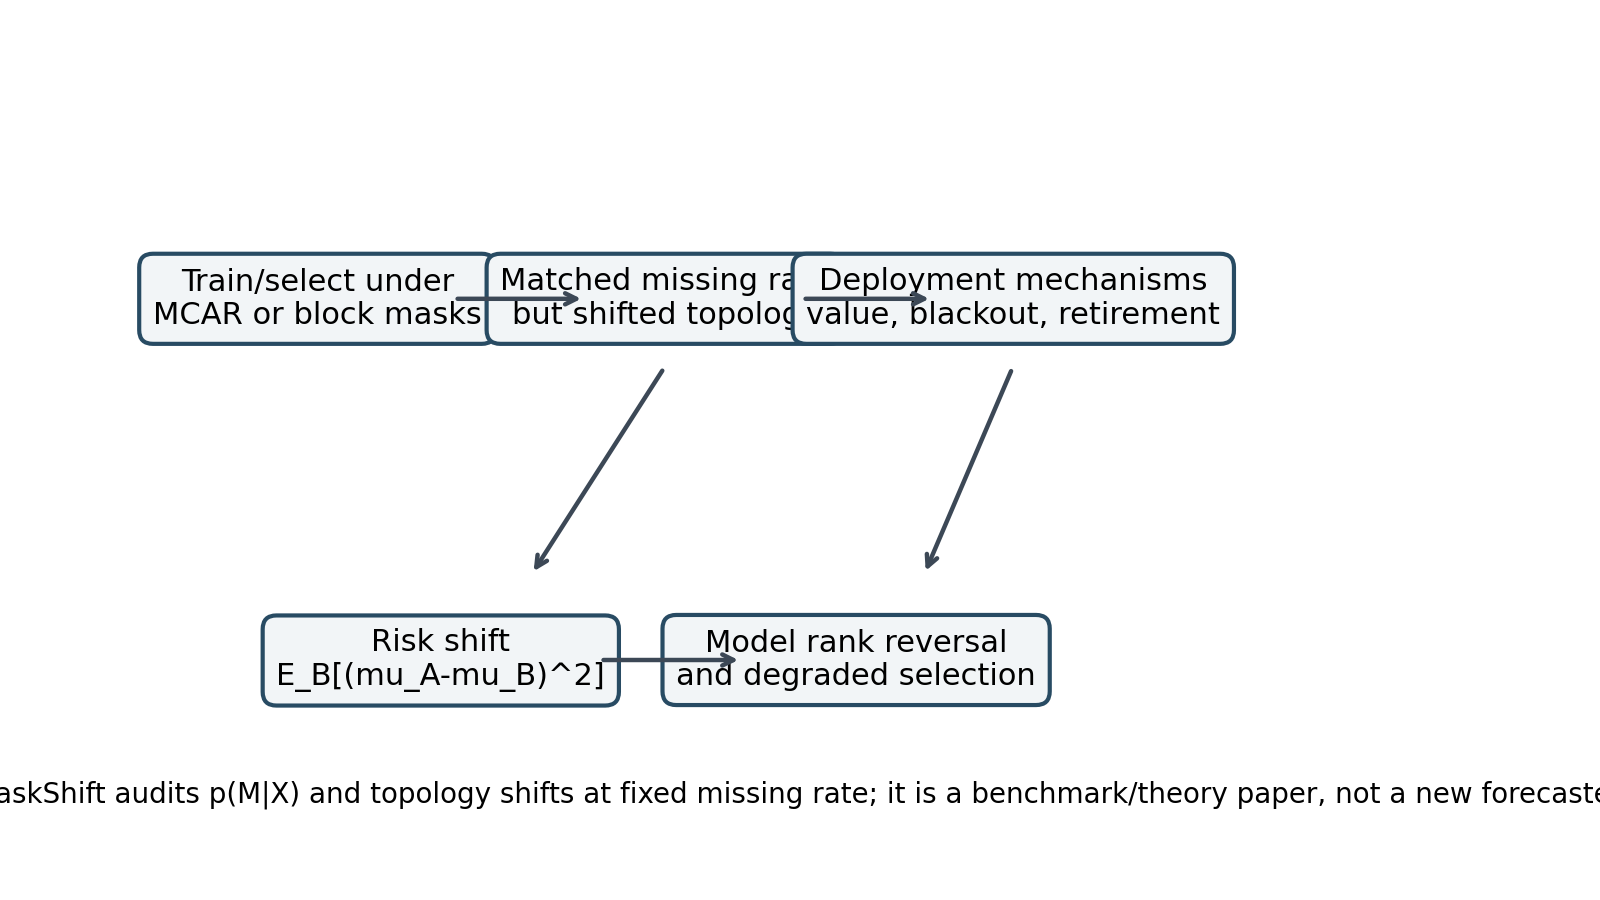
\includegraphics[width=.98\linewidth]{../figures/maskshift_overview.png}
\caption{MaskShift varies the conditional mask mechanism while controlling the marginal missing rate and keeping targets clean.}
\label{fig:overview}
\end{figure}

\section{Results}

\subsection{Mechanism Identity Explains Risk Shifts}

M1 trains under MCAR and tests under matched-rate operational mechanisms. Weather and Electricity pass the mechanism-shift gate. In the original four-dataset audit, Weather has eta-squared 0.614 and Electricity 0.777; Traffic and AirConvection do not pass the full gate. M10 repeats the core positive datasets over three seed offsets.

\begin{table*}[t]
\centering
\small
\begin{tabular}{lcccc}
\toprule
Dataset & $\eta^2$ mean [95\% CI] & Max deg. [95\% CI] & Worst $\tau$ [95\% CI] & Gate seeds\\
\midrule
Weather & 0.495 [0.000, 1.000] & 702.0\% [341.8, 1062.2] & 0.11 [-1.00, 1.00] & 2/3\\
Electricity & 0.572 [0.129, 1.000] & 175.1\% [129.3, 220.9] & -0.22 [-1.00, 1.00] & 3/3\\
\bottomrule
\end{tabular}
\caption{M1 multi-seed mechanism audit. The Weather confidence interval is wide; the paper therefore claims material evidence, not universal stability.}
\label{tab:m1}
\end{table*}

M13 adds a hierarchy-aware bootstrap over lightweight variants and test windows. The loss-shift result is stable on Weather and Electricity: max absolute delta has 95\% bootstrap intervals of 1.680 [0.514, 3.659] and 1.446 [0.862, 1.943], respectively. The same bootstrap is less decisive for rank instability, with rank-instability probabilities 0.46 and 0.53. We therefore anchor the rank-reversal claim primarily in the M9/M10 official-architecture result rather than in lightweight M1 ranks alone.

\subsection{The Result Is Not Only Retirement}

An easy reviewer objection is that retirement is too obvious. M8 removes this escape hatch. Weather and Electricity still pass when considering only value-triggered, volatility-triggered, and blackout mechanisms. Weather's strongest non-retirement mechanism is value-triggered missingness with 132.8\% degradation; Electricity's strongest non-retirement mechanism is also value-triggered missingness with 182.7\% degradation. Traffic and AirConvection fail this stricter gate.

\subsection{Official-Architecture Adaptation Shows Rank Reversal}

M9/M10 is the main model-facing result. PatchTST and TimeXer are imported from official TSLib model files and evaluated under MaskShift's custom encoder-mask protocol. This tests whether modern architecture classes are affected, without claiming a full official benchmark reproduction.

\begin{table*}[t]
\centering
\small
\begin{tabular}{lcccc}
\toprule
Dataset & Architectures & Max deg. [95\% CI] & Worst $\tau$ [95\% CI] & Gate seeds\\
\midrule
Weather & PatchTST, TimeXer & 135.8\% [8.6, 262.9] & -1.00 [-1.00, -1.00] & 3/3\\
Electricity & PatchTST, TimeXer & 128.6\% [98.1, 159.1] & -1.00 [-1.00, -1.00] & 3/3\\
\bottomrule
\end{tabular}
\caption{Official-architecture adaptation with TSLib PatchTST and TimeXer classes. The consistent $\tau=-1$ is direct evidence that MCAR model order need not transfer to operational mechanisms.}
\label{tab:m9}
\end{table*}

M16 extends official PatchTST/TimeXer coverage to the mixed datasets rather than leaving them as lightweight-model-only evidence. Traffic shows 35.4\% maximum degradation but worst Kendall $\tau=1.0$ and ANOVA $p=0.0854$; AirConvection shows 46.1\% maximum degradation but worst Kendall $\tau=1.0$ and ANOVA $p=0.000122$. Both are therefore mixed/negative for the rank-reversal gate. This strengthens the submission scope: mechanism shift is a benchmark factor whose strength is dataset- and architecture-dependent, not a universal rank-reversal theorem.

\begin{figure}[t]
\centering
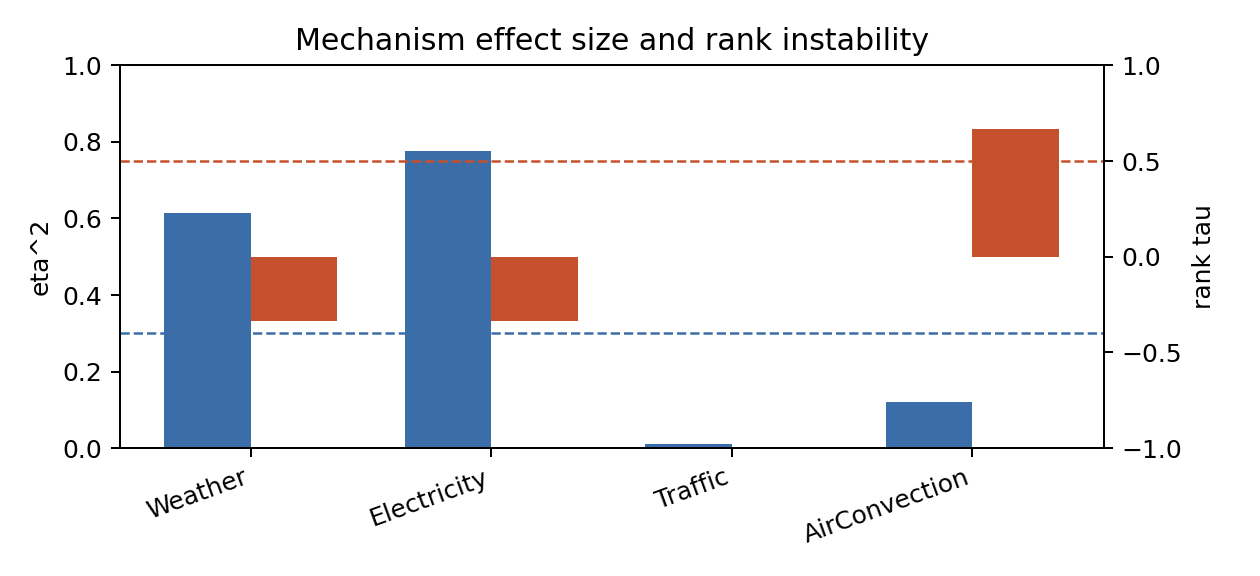
\includegraphics[width=.98\linewidth]{../figures/m1_mechanism_rank.png}
\caption{Mechanism effect size and rank instability under matched-rate masks.}
\label{fig:m1}
\end{figure}

\subsection{Missing-Aware Official Baselines}

M11 evaluates the official \texttt{ChannelTokenFormer\_missing} model class under the same MaskShift encoder-mask protocol. The result is mixed and useful: CTF\_missing is not simply broken by MaskShift, but neither does it eliminate mechanism sensitivity.

\begin{table*}[t]
\centering
\small
\begin{tabular}{lcccc}
\toprule
Dataset & Backbone & Max deg. [95\% CI] & Max abs. delta [95\% CI] & Gate seeds\\
\midrule
Weather & CTF\_missing & 96.0\% [39.4, 152.6] & 0.264 [0.003, 0.524] & 1/3\\
Electricity & CTF\_missing & 32.3\% [-10.4, 75.0] & 0.584 [-0.130, 1.297] & 0/3\\
\bottomrule
\end{tabular}
\caption{Official ChannelTokenFormer\_missing adaptation. Weather remains mechanism-sensitive, while Electricity is weaker and non-significant under the current sprint-time protocol.}
\label{tab:m11}
\end{table*}

M12 evaluates official S4M under the same reduced local protocol over three seed offsets. This is a negative/contrastive result rather than a positive mechanism-shift result: S4M does not pass the mechanism-shift gate in any seed.

\begin{table*}[t]
\centering
\scriptsize
\begin{tabular}{llcccc}
\toprule
Dataset & Backbone & Max deg. [95\% CI] & Max abs. [95\% CI] & $p$ [95\% CI] & Gate seeds\\
\midrule
Weather & S4M & 5.7\% [-44.9, 56.3] & 0.071 [-0.620, 0.762] & 0.509 [0.081, 0.938] & 0/3\\
Electricity & S4M & 6.2\% [-0.1, 12.5] & 0.312 [0.093, 0.530] & 0.933 [0.727, 1.000] & 0/3\\
\bottomrule
\end{tabular}
\caption{Official S4M adaptation over three seed offsets. S4M is a negative/contrastive missing-aware baseline under the reduced MaskShift protocol, so the paper does not claim that all missing-aware architectures are mechanism-sensitive.}
\label{tab:m12}
\end{table*}

Together, M11 and M12 change the submission posture. The paper no longer says that missing-aware official baselines are absent. Instead, it reports architecture-dependent evidence: CTF\_missing remains sensitive on Weather, while S4M is comparatively robust across three reduced local seed offsets. M14 doubles the S4M reduced setting to 16 channels, 64 train windows, and 48 test windows; the conclusion does not flip, with 0/3 gate seeds on both Weather and Electricity. In M14, Weather has 6.8\% [-8.8, 22.4] max degradation, 0.109 [-0.134, 0.352] max absolute delta, and Kruskal p 0.673 [0.000, 1.000]; Electricity has 2.5\% [-17.9, 22.8] max degradation, 0.154 [-1.382, 1.690] max absolute delta, and Kruskal p 0.989 [0.963, 1.000]. This weakens the critique that the S4M contrast is only an eight-channel artifact, while still falling short of, and not a full S4M benchmark reproduction.

\subsection{Corrected Severity Curves}

M7 originally exposed large denominator-driven relative-ratio spikes. M10 therefore adds absolute delta, log ratio, and symmetric relative delta. Table~\ref{tab:m7} supports a qualitative severity trend without relying on an unstable headline ratio.

\begin{table*}[t]
\centering
\small
\begin{tabular}{lccccc}
\toprule
Rate & $\eta^2$ [95\% CI] & Abs. delta [95\% CI] & Log ratio [95\% CI] & Sym. delta [95\% CI] & Unstable\\
\midrule
0.10 & 0.194 [0.000, 0.456] & 0.540 [0.225, 0.855] & 0.66 [0.01, 1.30] & 0.62 [0.06, 1.17] & 0/4\\
0.20 & 0.286 [0.000, 0.657] & 10.713 [-22.257, 43.683] & 1.33 [-1.55, 4.22] & 0.80 [-0.45, 2.05] & 0/4\\
0.35 & 0.423 [0.000, 0.881] & 2.577 [-3.801, 8.954] & 1.27 [-0.40, 2.94] & 0.98 [-0.16, 2.11] & 0/4\\
0.50 & 0.472 [0.060, 0.884] & 0.854 [0.452, 1.256] & 0.92 [0.01, 1.83] & 0.82 [0.13, 1.51] & 0/4\\
\bottomrule
\end{tabular}
\caption{Corrected robustness metrics by missing rate. M7 corrected metrics use one seed across all four datasets/rates in the sprint-time hardening run.}
\label{tab:m7}
\end{table*}

\subsection{Typed Head Negative Result}

The typed/topology head was tested as a minimal correction. It does not pass the paper's method gate. Weather improves by 22.9\%, but Electricity improves by only 3.3\%, Traffic worsens by 5.6\%, and AirConvection improves by 7.5\%. The overall typed improvement test has $p=0.214$. The correct interpretation is not that MaskShift proposes a new typed head; it is that mechanism labels and topology statistics are plausible diagnostics, but the current lightweight correction is not a robust solution.

\begin{figure}[t]
\centering
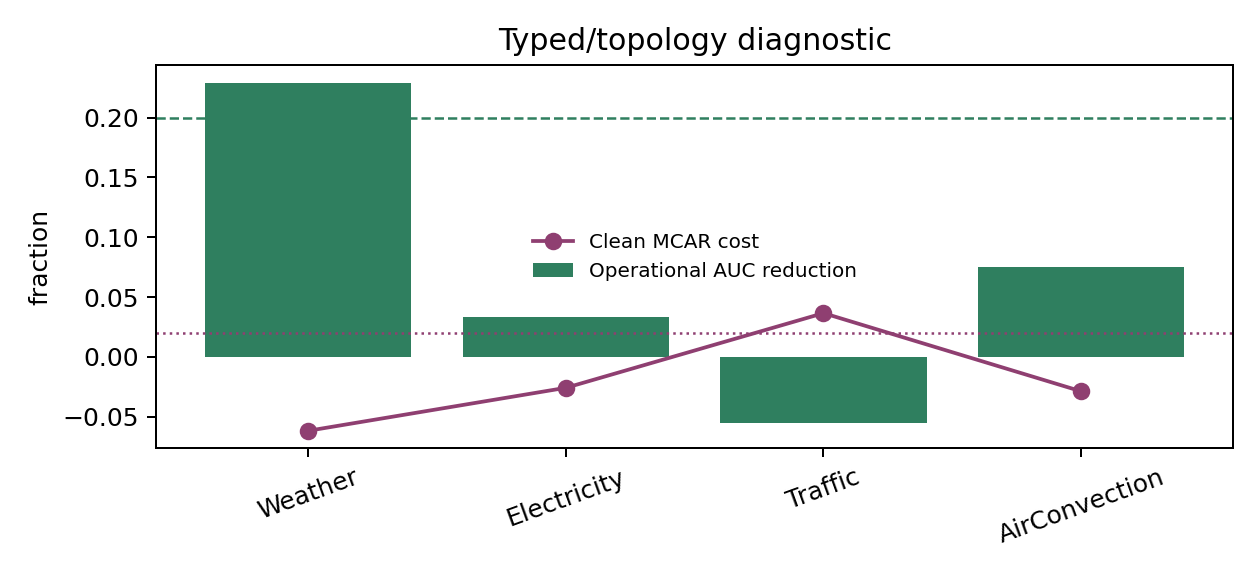
\includegraphics[width=.98\linewidth]{../figures/m2_typed_correction.png}
\caption{Typed/topology diagnostic versus topology-only baseline. H3 fails and is reported as a negative result.}
\label{fig:m2}
\end{figure}

\section{Related Work}

GRU-D established that missingness masks and time gaps can carry predictive information in recurrent models~\cite{che2018grud}. BRITS~\cite{cao2018brits} and diffusion approaches such as CSDI~\cite{tashiro2021csdi} and SADI~\cite{islam2025sadi} focus on imputation or joint reconstruction. SADI is especially relevant because it studies partial blackout scenarios, but its target is imputation quality under blackout-like patterns rather than model selection under matched-rate mechanism shift.

S4M~\cite{jing2025s4m} and ChannelTokenFormer~\cite{jang2026channeltokenformer} are closer architecture-level competitors. S4M designs missing-aware state-space forecasting, while ChannelTokenFormer targets dependency, asynchrony, and missingness in a unified framework. MaskShift is intentionally orthogonal: it is useful even if a missing-aware architecture wins, because it asks whether the evaluation protocol controls the right factor.

Modern TSF backbones such as DLinear~\cite{zeng2023dlinear}, PatchTST~\cite{nie2023patchtst}, iTransformer~\cite{liu2024itransformer}, and TimeXer~\cite{wang2024timexer} define the architecture context for the benchmark. Irregular-sampling forecasting methods such as GraFITi~\cite{yalavarthi2024grafiti} address a different data-acquisition axis from matched-rate mechanism shift. CRIB/MTSF-M~\cite{yang2025crib} motivates direct forecasting from partially observed series. Robust prediction under missingness shifts~\cite{rockenschaub2024missingness} gives a statistical anchor outside TSF. The information-blackout preprint~\cite{sunesh2026blackouts} is the closest task collision because it models MNAR traffic blackouts, but MaskShift broadens the question from a single blackout model to multiple mechanisms and model-rank stability.

\section{Limitations}

The strongest evidence is concentrated on Weather and Electricity. Traffic and AirConvection are included precisely because they weaken any universal claim. M9 imports official TSLib model classes, but it does not reproduce the full official TSLib benchmark protocol; it uses custom windows, custom masks, reduced training samples for multi-seed feasibility, and encoder-input-only corruption. M11 integrates official ChannelTokenFormer\_missing and M12/M14 integrate official S4M, but both runs are adaptations under MaskShift windows, masks, reduced samples, and local compute limits. M12 uses three seed offsets and M14 doubles channels and train/test windows, but neither reproduces the full S4M benchmark protocol or full-channel setting. M10/M11/M12/M14 confidence intervals use only three seed offsets, and M13 bootstraps variants/windows rather than a full hierarchy over series, horizons, seeds, and datasets. These are sprint-time robustness summaries rather than final large-sample inference. Finally, the typed-head correction fails the method gate, ruling out a method-paper framing.

\section{Conclusion}

MaskShift identifies an under-controlled failure mode in missing-value forecasting evaluation. Matching the missing rate does not match the conditional mask mechanism. When the mechanism shifts, forecast risk and model rankings can shift as well. The current evidence supports a benchmark/theory submission: Weather and Electricity show strong mechanism sensitivity, official PatchTST and TimeXer architecture classes show rank reversal under the MaskShift protocol, ChannelTokenFormer\_missing adds mixed missing-aware evidence, S4M adds a useful negative/contrastive missing-aware baseline, and non-retirement mechanisms are sufficient to produce material degradation. The honest submission scope is narrow but useful: report missingness mechanism and topology as first-class benchmark factors, do not certify deployment missingness robustness from MCAR/block tests alone, and treat the failed typed head as a diagnostic negative result rather than a method contribution.

\bibliographystyle{plain}
\bibliography{references}
\end{document}
